\section{Regularization}
\script{203} Dabei werden die Parameter vom Modell nicht mit Least Square gesucht, sondern mit anderen Verfahren. Diese können unter umständen bessere Werte liefern. Zwei bekannte Vertreter sind:
\begin{itemize}
	\item Ridge Regression
	\item Lasso Regression
\end{itemize}

Dabei wird ein zusätzlicher Faktor $\lambda$ eingeführt, um die Optimierung zu steuern. Hauptunterschied ist, dass bei der Rdige Regression keine Koeffizienten mit 0 Auftretten können.
\begin{center}
	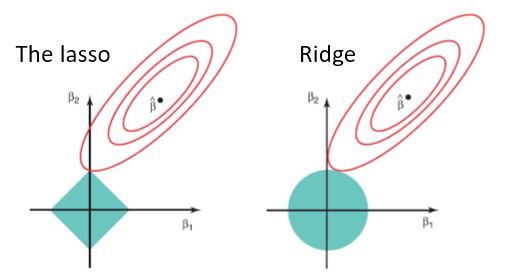
\includegraphics[width=0.5\columnwidth]{./Images/lasse}
	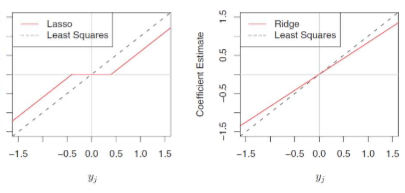
\includegraphics[width=0.5\columnwidth]{./Images/lasse_2}
\end{center}

\subsection{Normalization}
Ziel von der Normalizierung ist es, die Daten ohne Offset zu haben ($\beta_0 = 0$)